\documentclass[12pt]{article}
\bibliographystyle{plain}

\usepackage{hyperref}
\usepackage[sc]{mathpazo}
\usepackage[utf8]{inputenc}
\usepackage{graphicx}
\usepackage{subfigure}
\pagestyle{empty}
\oddsidemargin=0in
\evensidemargin=0in
\topmargin=-.5in
\textwidth=6.5in
\textheight=9.2in

\title
{tICA Tutorial}

\author{Christian Schwantes}

\begin{document}

\maketitle

\tableofcontents
%\section{Table of Contents}
%\begin{enumerate}
%\item Introduction of tICA
%\item tICA Tutorial within MSMBuilder
%\item Selection of tICA Parameters
%\item Analyzing the tICs
%\item Drawbacks of tICA
%\end{enumerate}

\newpage
\section{Introduction of tICA}

The contents of this document will build on concepts introduced in the MSMBuilder Tutorial. We will assume the reader is familiar with those ideas.

The time-structure based Independent Component Analysis (tICA) method as applied to MSM construction is a new way to judge distances in the protein conformational landscape. tICA can be built as an adaptation of Principal Component Analysis (PCA).

In PCA, the goal is to find projection vectors that maximize their explained variance, subject to them being uncorrelated and having length one. In tICA, the goal is to find projection vectors that maximize their autocorrelation function, subject to them being uncorrelated and having unit variance. It is easy to show (see Schwantes, CR and Pande, VS. {\it JCTC} {\bf 2013}, 2000-2009.) that the solution to the tICA problem are the solutions to this eigenproblem:
$$ C^{(\Delta t)} v = \lambda \Sigma v $$ If we represent each conformation in our trajectory as a vector in $\mathbb{R}^d$ (denote such a conformation as $\mathbf{X}(t)$), then we define:
$$ C^{(\Delta t)}_{ij} = \mathbb{E}\Big[ X_i(t) X_j(t+\Delta t) \Big] $$
$$ \Sigma_{ij} = \mathbb{E}\Big[ X_i(t) X_j(t) \Big] $$ $C^{(\Delta t)}$ is referred to as the time-lag correlation matrix, and $\Sigma$ is the covariance matrix.

Given this solution, we can use the tICA method to define a reduced dimensionality representation of each $\mathbf{X}(t)$ by projecting the vector onto the slowest $n$ tICs. Therefore, the strategy for using tICA to construct an MSM looks like:

\begin{enumerate}
\item Calculate $C^{(\Delta t)}$ and $\Sigma$ and the solutions to the generalized eigenvalue problem given above
\item Choose the number of tICs to project onto
\item Use the reduced space to cluster and assign conformations to states
\item Build the MSM from these assignments and analyze as laid out in the MSMBuilder tutorial
\end{enumerate}

In the next section we will go over how to do each of these steps within MSMBuilder.

\section{tICA Tutorial within MSMBuilder}

Currently, the necessary library functions and scripts can be found in Christian Schwantes's fork of MSMBuilder hosted at \url{www.github.com/schwancr/msmbuilder} in the branch \texttt{tica\_mle}. 

The first step is to clone and install this branch:

\begin{verbatim}
$ mkdir schwancr_msmb
$ cd schwancr_msmb
$ git clone git@github.com:schwancr/msmbuilder
$ cd msmbuilder
$ git checkout tica_mle
$ python setup.py install
\end{verbatim}

This fork has everything you should need from MSMBuilder and more, so you can do everything you could have done with the main branch.

\subsection{Calculate $C^{(\Delta t)}$ and $\Sigma$ and the tICs}

The first step is to calculate the time-lag correlation and covariance matrices. The script that does this is \texttt{tICA\_train.py}, which will calculate the matrices, find the eigenvectors, and save all results.

At this point, we need to select a $\Delta t$. Currently, there is no automated procedure for selecting it, but for most systems the value has not changed the results drastically. In the past, values in the range of 10s to 100s of nanoseconds have worked well for protein folding simulations with timescales in the micro to milliseconds. We suggest using a range and comparing the resulting MSMs' timescales to choose this parameter.

REMEMBER: All parameters that are times should be input in units of frames. This is true for all MSMBuilder scripts/libraries.

The \texttt{tICA\_train.py} script must be told how you want to represent each conformation as a vector. Since translation and rotation cannot be handled well with tICA (or PCA for that matter) we must use some internal representation of the conformation. We will define these by using one of the metrics within MSMBuilder:
\begin{enumerate}
\item Dihedral - $\sin$ and $\cos$ of all dihedral angles 
\item ContinuousContact - distances between pairs of residues
\item AtomPairs - distances between pairs of atoms
\end{enumerate} You should read about these, but we will use the AtomPairs representation in the following example.

The AtomPairs metric represents each conformation by a vector corresponding to the distance between pairs of atoms. We will use the following atom pairs for this representation (in AtomPairs.dat):

\begin{verbatim}
$ cat HeavyAtomPairs.dat
5 4
6 4
6 5
...
16 14
16 15
\end{verbatim}
Change to the reference folder of the msmbuilder package. Then run the following command:
\begin{verbatim}
$ tICA_train.py -d 10 -p ProjectInfo.yaml -s 1 -o tICAData.h5 atompairs 
                -a HeavyAtomPairs.dat
\end{verbatim} This will produce the file tICAData.h5 which is a serialized dictionary. You can read it with \texttt{msmbuilder.io.loadh}. The dictionary has the following keys:
\begin{enumerate}
\item \texttt{vals} - eigenvalues from the eigenvalue problem
\item \texttt{vecs} - eigenvectors from the eigenvalue problem normalized to unit variance; each column is an eigenvector
\item \texttt{cov\_mat} - covariance matrix ($\Sigma$)
\item \texttt{timelag\_corr\_mat} - time lag correlation matrix ($C^{(\Delta t)}$)
\end{enumerate} 

\subsection{Cluster and Assign Using $n$ tICs}
Now that we have the tICs calculated, we just need to use them when clustering. At this point, however, we need to decide how many tICs to use in the clustering step. The value of using the tICA method is to ignore degrees of freedom that only add noise to the distance calculation, so the resulting MSM will be qualitatively different depending on the choice here. 

{\it At this point there is no optimal way to choose the number of tICs to project onto. We suggest building many models over a range of $n$ from five to 30, and comparing the resulting MSMs. See the next section for a discussion of the effect of these parameters.}

We use the same scripts used in the regular MSMBuilder pipeline. To cluster the data (subsampled every 10 frames) and output the generators we do:
\begin{verbatim}
$ Cluster.py -p ProjectInfo.yaml -s 10 -o Data tica --po tICAData.h5 --nv 3 
             atompairs -a HeavyAtomPairs.dat kcenters -k 50
\end{verbatim} Notice that it appears that we are inputing two metrics (tica and atompairs). The reason is that tica requires us to specify the underlying metric used to turn the conformation into a vector. It is important, therefore, that we use the same metric here as we did in the \texttt{tICA\_train.py} step.

Now that we have the generators output, we do the assign step in an analogous use of \texttt{Assign.py}:
\begin{verbatim}
$ Assign.py -p ProjectInfo.yaml -g Data/Gens.lh5 -o Data/ tica --po 
            tICAData.h5 --nv 3 atompairs -a HeavyAtomPairs.dat
\end{verbatim} 

Now that we have an \texttt{Assignments.h5} file the remainder of the analysis can follow the pipeline described in the MSMBuilder tutorial.

\section{Selection of tICA Parameters}

There are two parameters introduced in the tICA method. The first is $\Delta t$, which is used in the calculation of the time-lag correlation matrix ($C^{(\Delta t)}$). The second is $n$, which is the number of tICs to project onto when calculating distances between conformations. 

There is currently no optimal method for choosing these parameters, however, the method has been fairly robust to different choices. 

In previous analyses of Fip35, villin, NTL9(1-39), and NuG2, $\Delta t$ between 50 and 1000 nanoseconds produced MSMs with largely the same timescale distribution, indicating that something in this range should be appropriate for most protein systems.

MSMs are more sensitive, however, to the selection of the number of tICs to project onto. In the previous analyses listed above, we found that using a surprisingly small number (in the range of 5-20) of tICs worked well. The power behind tICA is to ignore the degrees of freedom that quickly decorrelate and only add noise in the distance calculation.

However, as $n$ gets smaller, the resolution of the MSM becomes only able to discern conformations along the slowest coordinate (which is often the folding process). 

For example, in our analysis of NTL9, we found that increasing $n$ from three up to seven kept the folding timescale largely unchanged but added new microsecond timescales to the resulting MSMs, while adding in too many (< 10) produced a folding timescale that was too fast.

\section{Understanding the tICs}

The top tICs represent linear combinations of the input degrees of freedom that decorrelate slowly. These vectors are not necessarily easy to visualize, however.

For instance, the slowest tIC from the above analysis can be visualized as a matrix, where each entry corresponds to the tIC entry corresponding to a pair of atoms' distances.
\begin{figure}[h!]
\centering{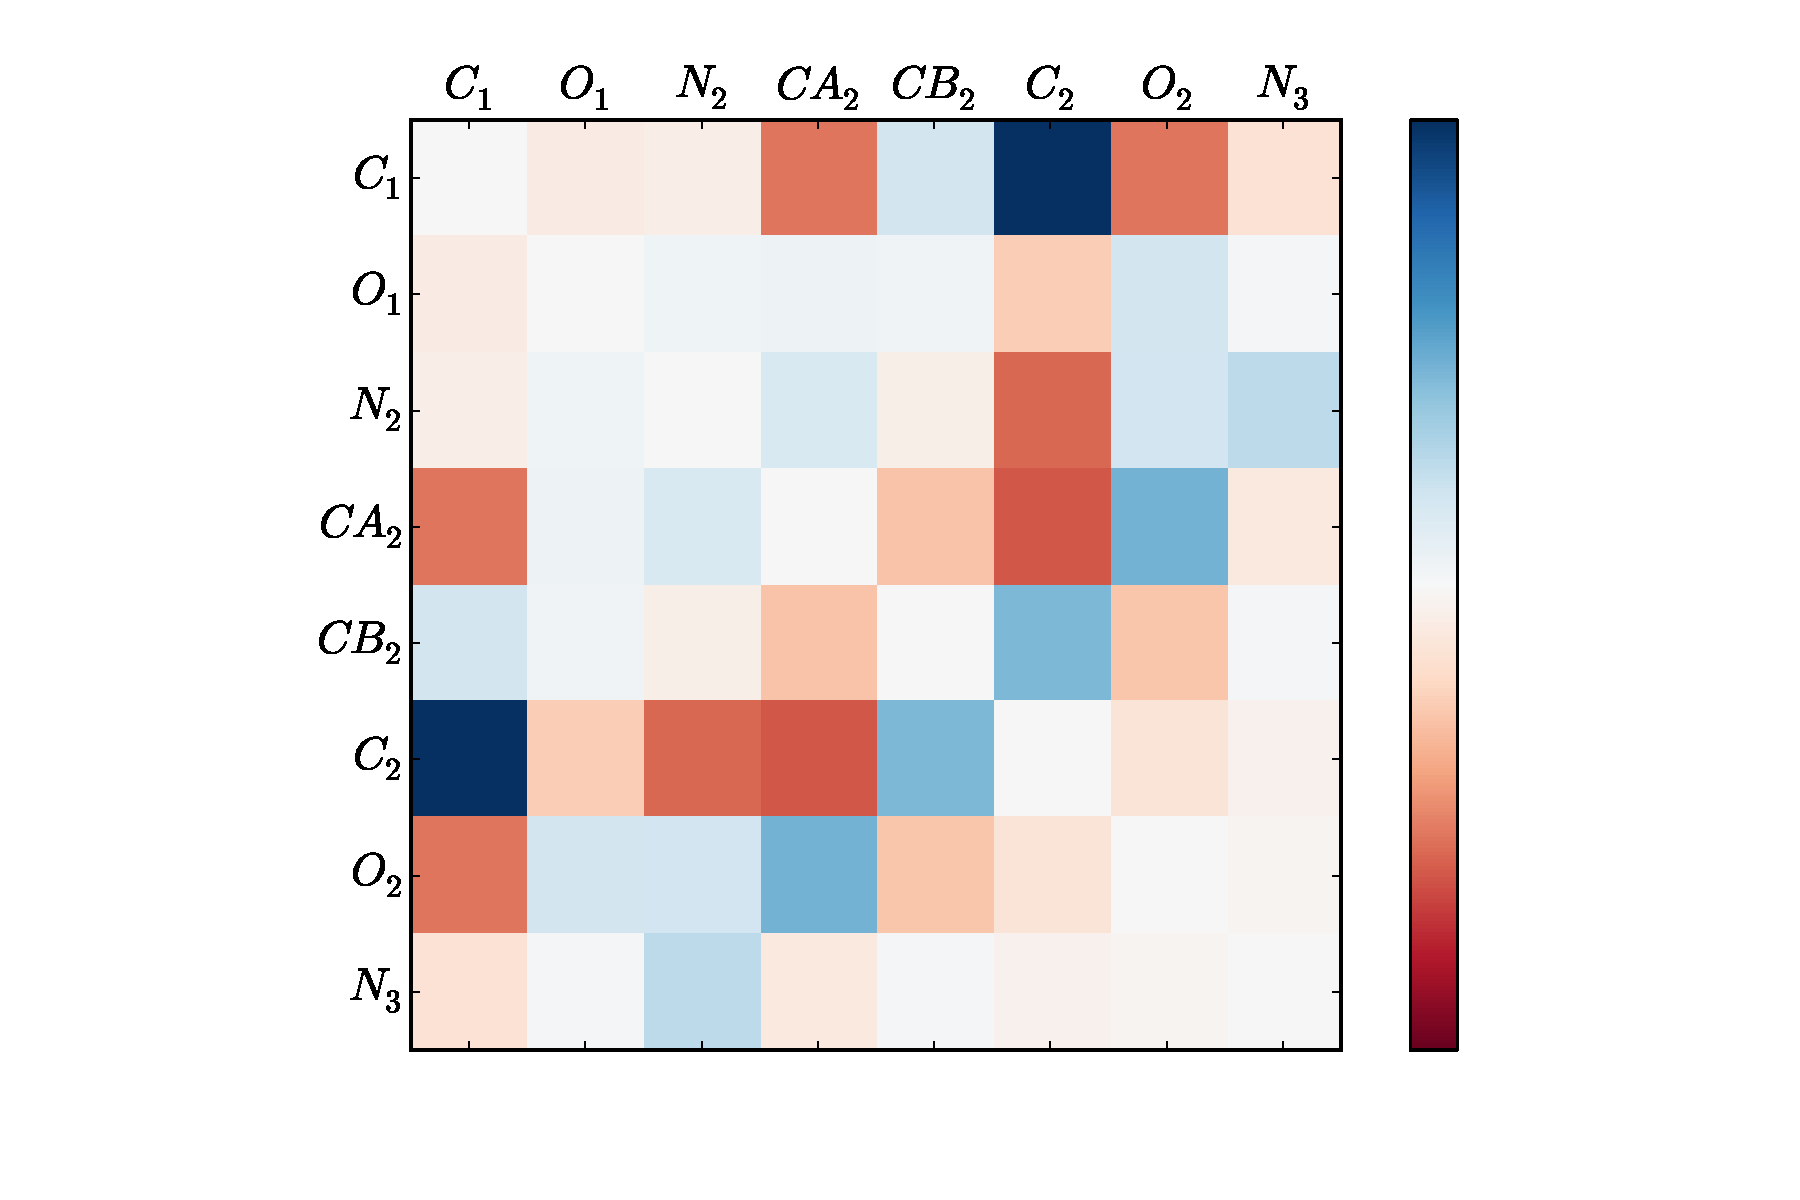
\includegraphics[width=4in]{tic0.pdf}}
\end{figure} Here, the dark blue and dark red portions correspond to atom pairs that best distinguish between far regions along the first tIC. As is clear, this is not all that helpful to look at (though an area that could be greatly improved is providing a visualization tool for these degrees of freedom).

We can also attempt to visualize the tICs by comparing the projections onto each tIC to order parameters. For instance, for each conformation we sampled in the reference simulations, we can calculate the phi and psi angles along with the projection of the conformation onto each tIC. In this way, we can visualize what each tIC corresponds to.

\begin{figure}[h!]
\centering{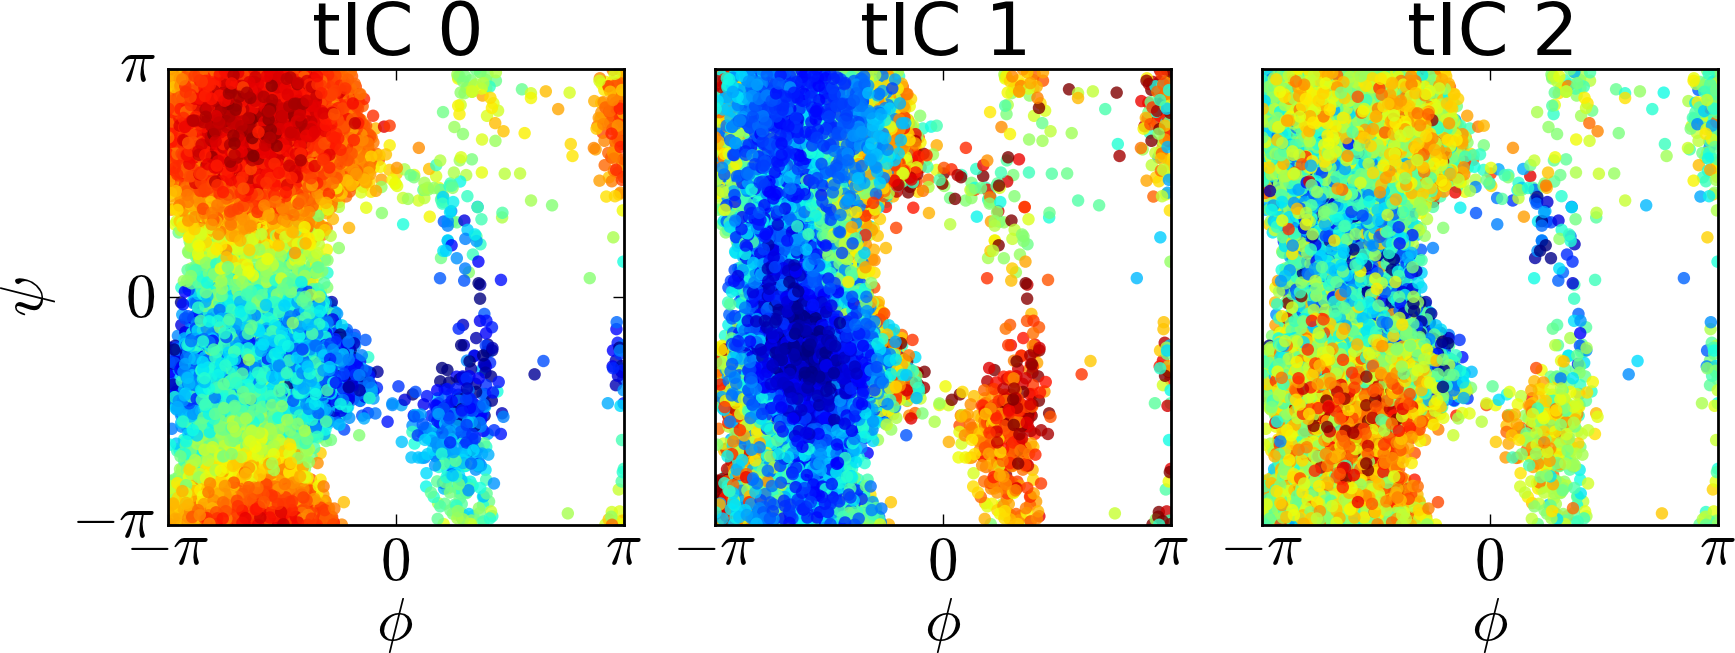
\includegraphics[width=6in]{tics_crop.png}}
\end{figure}

\section{Drawbacks of tICA}

Since part of the process of using tICA is a dimensionality reduction, there is always the opportunity to throw out important pieces of information. In particular, by throwing out the faster degrees of freedom, we can better estimate the slowest timescales; but this comes with the trade-off of not representing the fast timescales correctly. The result is illustrated when trying to sample a trajectory from the MSM built on tICA. The result is a trajectory that represents the folding/unfolding transition well, but when in the unfolded state jumps around more than would be seen in a typical MD simulation.

\bibliography{Tutorial}


\end{document}
